\documentclass{article}
\usepackage[left=1.9cm,top=2.4cm,right=2.4cm,bottom=2cm]{geometry} 
\usepackage[spanish]{babel}
\usepackage[utf8]{inputenc}
\usepackage{amsmath}
\usepackage{amsfonts}
\usepackage{amssymb}
\usepackage{verbatim}
\usepackage{url}
\usepackage{graphicx}
\usepackage{float}
\usepackage{enumerate} % To use different item symbols in enumerate
\usepackage[inline]{enumitem} % To use different item symbols in enumerate
\usepackage{multicol} % multicolumns
\usepackage{fancyhdr}%Header and Footers
\pagestyle{fancy}
\fancyhf{}
\chead{Universidad Nacional de Colombia\\
Taller I}
\cfoot{\thepage}
\renewcommand{\headrulewidth}{0pt} %remove header line
%\renewcommand{\footrulewidth}{1pt} % set footer line

\title{Universidad Nacional de Colombia\\ Fundamentos de Electricidad y Magnetismo\\ (PEAMA Sumapaz 2023-II)} %\normalsize{text} normal size of the text font
\author{\textbf{Taller I}} %\underline{text} hightlights the text with a line
%\date{\textbf{Nombre: \rule{12cm}{0.15mm}}}

\begin{document}
\maketitle

\renewcommand{\tablename}{Tabla}

\subsection*{INDICACIONES}
Las sesiones taller tiene como objetivo evaluar la compresión de diversas tematicas a través la expresión escrita. Por lo tanto, la solución de cada problema debe ser un texto expositivo bien redactado, esto incluye a las ecuaciones y procedimientos matemáticos ya que estos también son texto. Como texto la solución debe tener un propósito claro (calcular,explicar, identificar, describir, relacionar. . . ) ysu redacción debe ser siempre coherente con tal propósito.\\

Teniendo en cuenta lo anterior, los criterios de evaluación de las soluciones son los siguientes:
\begin{enumerate}[label=\roman*)]
\item  \textbf{Descripción de la situación:} Todo problema tiene un contexto o una situación específica. El estudiante debe realizar una descripción de tal contexto y hacer uso de un esquema o figura donde relaciones todos los conceptos, cantidades físicas y/o matemáticas del problema.
\item \textbf{Redacción de la solución:} Todo argumento dado por el estudiante debe ser claro, justificado y debidamente citado o referenciado con la información dada en las clases y/o desde bibliografía relacionada.
\item \textbf{Uso del lenguaje disciplinar y matemático:} Todos los conceptos físicos y matemáticos en la solución deben usarse bien (buen lenguaje y buen manejo de unidades físicas) y las ecuaciones deben ser parte del texto (no una lista de símbolos únicamente).
\item \textbf{Uso de esquemas y figuras:} El estudiante debe hacer buen uso de las imágenes, es decir que debe usar la imagen dentro del texto y todas las variables y/o cantidades que se encuentren en la imagen debe ser definidas en el texto principal.
\end{enumerate}

Las soluciones a los problemas deben ser entregadas de forma \textbf{individual} a lo largo de todo el semestre. 
\section*{PROBLEMAS}
\begin{enumerate}

\item Encuentre el gradiente de los siguientes campos escalares:

\begin{enumerate}
\item $f(x,y,z)=x^{2}+y^{3}+z^{4}.$
\item $f(x,y,z)=x^{2}y^{3}z^{4}.$
\item $f(x,y,z)=e^{x}\sin(y)\ln(z).$
\end{enumerate}

\item Calcule la divergencia de los siguientes campos vectoriales:
\begin{enumerate}
\item $\vec{F}_{a}=(x^{2},3xz^{2},-2xz)$.
\item $\vec{F}_{a}=(xy,2yz,3zx)$.
\end{enumerate}
\pagebreak
\item Suponga que el campo de la figura \ref{rot-div}a es $\vec{F}_{a}=(-y,x,0)$ y el de la figura \ref{rot-div}b es $\vec{F}_{b}=(0,x,0)$.

\begin{figure}[H]
\centering
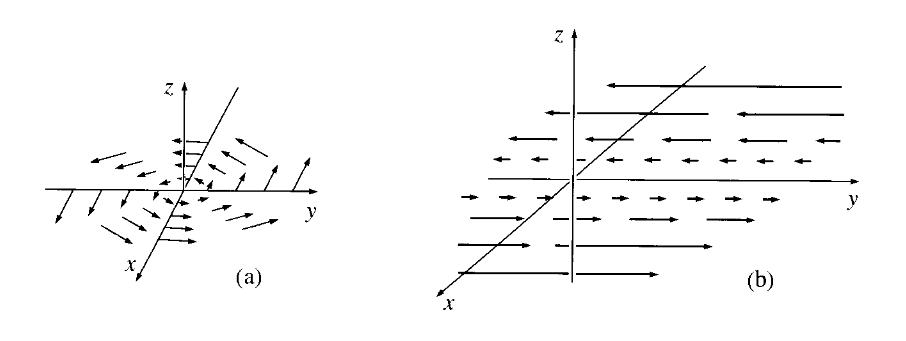
\includegraphics[scale=0.5]{rotacional-divergencia.png}
\caption{Campos vectoriales problema 3.}
\label{rot-div}
\end{figure}

Calcule la divergencia y el rotacional de cada campo e interprete sus resultados.

\item Calcule la integral de línea para el campo $\vec{F}=(y^2,2x(y+1),0)$ desde el punto $\vec{a}=(1,1,0)$ hasta el punto $\vec{b}=(2,2,0)$ a lo largo de la curva (1) de la figura \ref{int_linea}.

\begin{figure}[H]
\centering
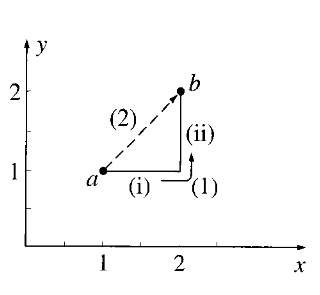
\includegraphics[scale=0.5]{int_linea.png}
\centering 
\caption{Diagrama integral de línea problema 4.}
\label{int_linea}
\end{figure}

\textbf{NOTA:} La curva (1) está compuesta de dos líneas: línea (i) y línea (ii). Además, tenga en cuenta que:

\begin{itemize}
\item para (i): $y=1$ y $d\vec{\ell}_{i}=dx$
\item para (ii): $x=2$ y $d\vec{\ell}_{ii}=dy$
\end{itemize}
\pagebreak
\item Calcule la integral de superficie del campo $\vec{F}=(2xz,(x+2),y(z^{2}-3))$ a través de las cinco caras (excluyendo la cara de abajo) de la caja mostrada en la figura \ref{int_superficie}.

\begin{figure}[H]
\centering
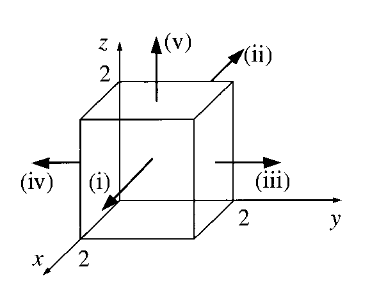
\includegraphics[scale=0.5]{int_superficie.png}
\centering 
\caption{Diagrama integral de superficie problema 5.}
\label{int_superficie}
\end{figure}

\textbf{NOTA:} Tenga en cuenta los vectores (i), (ii), (iii), (iv) y (v) son los vectores normales a la superficie y con ellos puede definir los diferenciales de superficie de cada cara de la caja. Por ejemplo, note que el diferencial de superficie de las caras (iii) y (iv) son respectivamente:

\begin{align*}
d\vec{S}_{iii}&=\hat{y}dxdz,\\
d\vec{S}_{iv}&=-\hat{y}dxdz.
\end{align*}

\end{enumerate}
\end{document}
